
\section{Domain Driven Design (8P)}
\subsection{Ubiquitous Language (2P)}
\task{4 Beispiele für die Ubiquitous Language; jeweils Bezeichung, Bedeutung und kurze Begründung, warum es zur Ubiquitous Language gehört}

\begin{table}[H]
\begin{tabular}{|l|l|l|}
\hline
Bezeichung &
  Bedeutung &
  Begründung \\ \hline
Bank Account &
  \begin{tabular}[c]{@{}l@{}}Ein Finanzkonto, das von einem \\ Kunden genutzt wird, um Geld \\ zu speichern und zu verwalten.\end{tabular} &
  \begin{tabular}[c]{@{}l@{}}Ein "Bank Account" ist die zentrale Entität, \\ um Guthaben, Einzahlungen und Abhebungen \\ zu verfolgen. Es ist ein grundlegendes Konzept \\ in Bilanzius.\end{tabular} \\ \hline
Transaction &
  \begin{tabular}[c]{@{}l@{}}Eine finanzielle Aktivität, bei \\ dem Geld zwischen Konten bewegt \\ wird, dazu gehören Einzahlungen \\ und Abhebungen.\end{tabular} &
  \begin{tabular}[c]{@{}l@{}}Transaktionen stellen die grundlegenden \\ Operationen dar, die den Zustand eines \\ Kontos verändern.\end{tabular} \\ \hline
Balance &
  \begin{tabular}[c]{@{}l@{}}Der Betrag an Geld, der aktuell \\ auf einem Bankkonto verfügbar ist.\end{tabular} &
  \begin{tabular}[c]{@{}l@{}}Die "Balance" gibt den aktuellen Stand \\ eines Kontos an und ist entscheidend, \\ um zu bestimmen, ob weitere \\ Transaktionen durchgeführt werden können.\end{tabular} \\ \hline
Report &
  \begin{tabular}[c]{@{}l@{}}Ein Dokument, das die Transaktionen \\ eines Bankkontos über einen \\ bestimmten Zeitraum zusammenfasst.\end{tabular} &
  \begin{tabular}[c]{@{}l@{}}Der "Report" gibt dem Kunden eine detaillierte \\ Übersicht über alle Aktivitäten auf seinem Konto, \\ einschließlich Einzahlungen und Abhebungen. \\ Es hilft bei der Überwachung der Finanzen.\end{tabular} \\ \hline
\end{tabular}
\end{table}
 
\subsection{Repositories (1,5P)}
\task{UML, Beschreibung und Begründung des Einsatzes eines Repositories; falls kein Repository vorhanden: ausführliche Begründung, warum es keines geben kann/hier nicht sinnvoll ist – NICHT, warum es nicht implementiert wurde} 
Der BankAccountService ist ein, obwohl er ungünstig benannt wurde, Repository. Dieses ermöglicht den Zugriff auf die BankAccount Datenschicht. Es stellt einfache CRUD Operationen bereit.

\begin{figure}[htbp]
    \centering
    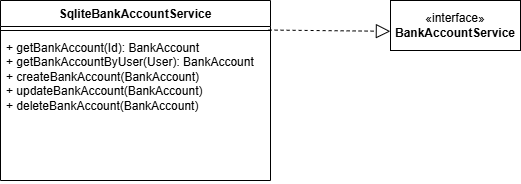
\includegraphics[width=\linewidth]{kapitel6_ddd/repo.png}
\end{figure}

\subsection{Aggregates (1,5P)}
\task{UML, Beschreibung und Begründung des Einsatzes eines Aggregates; falls kein Aggregate vorhanden: ausführliche Begründung, warum es keines geben kann/hier nicht sinnvoll ist– NICHT, warum es nicht implementiert wurde} 
Ein Aggregate ist eine Gruppe von eng zusammengehörigen Domain-Objekten, die im System als eine logische Einheit betrachtet und behandelt wird. Im Zentrum steht der sogenannte Aggregate Root, der als einziger Zugangspunkt zu den enthaltenen Objekten dient. Das BankAccountAggregate erlaubt den Zugriff auf ein BankAccount Entity. Es kapselt die \textit{setBalance} Funktion und ermöglicht so eine bessere Integritätsprüfung.
\begin{figure}[htbp]
    \centering
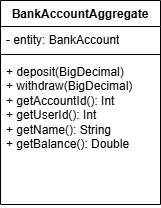
\includegraphics{kapitel6_ddd/aggregate.drawio.png}
\end{figure}
\newpage
\subsection{Entities (1,5P)}
\task{UML, Beschreibung und Begründung des Einsatzes einer Entity; falls keine Entity vorhanden:  
ausführliche Begründung, warum es keine geben kann/hier nicht sinnvoll ist– NICHT, warum es nicht implementiert wurde}
Das Entity BankAccount repräsentiert ein Java-Objekt, das der Datenbanktabelle BankAccount entspricht. Es ermöglicht einen unkomplizierten und direkten Zugriff auf die darin gespeicherten Daten aus dem Java-Code heraus.
\begin{figure}[htbp]
    \centering
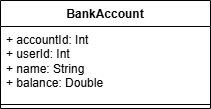
\includegraphics{kapitel6_ddd/entity.png}
\end{figure}
\newpage
\subsection{Value Objects (1,5P)}
\task{UML, Beschreibung und Begründung des Einsatzes eines Value Objects; falls kein Value Object vorhanden: ausführliche Begründung, warum es keines geben kann/hier nicht sinnvoll ist– NICHT, warum es nicht implementiert wurde}
Die Klasse \textit{HashedPassword} ist als Value Object für Passwörter konzipiert. Sie macht deutlich, dass das darin enthaltene Passwort ausschließlich in gehashter Form vorliegt und nicht im Klartext gespeichert sind. Dadurch soll sichergestellt werden, dass es während der Entwicklung nicht zu Missverständnissen im Umgang mit Passwörtern kommt.
\begin{figure}[htbp]
    \centering
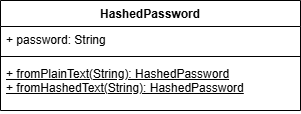
\includegraphics{kapitel6_ddd/valueobject.drawio.png}
\end{figure}